\documentclass[14pt,a4paper]{extarticle}

\usepackage{fontspec}
\usepackage{polyglossia}
\setmainlanguage{russian}
\setotherlanguage{english}

\setmainfont[Ligatures=TeX]{Times New Roman}
\setsansfont[Ligatures=TeX]{Arial}
\setmonofont{Consolas}

\newfontfamily\cyrillicfont[Ligatures=TeX]{Times New Roman}
\newfontfamily\cyrillicfontsf[Ligatures=TeX]{Arial}
\newfontfamily\cyrillicfonttt{Consolas}

\usepackage{geometry}
\geometry{
    left=30mm,
    right=15mm,
    top=20mm,
    bottom=20mm
}

\usepackage{setspace}
\onehalfspacing

\usepackage{indentfirst}
\setlength{\parindent}{1.25cm}

\usepackage{amsmath}
\usepackage{amssymb}
\usepackage{graphicx}
\usepackage{float}
\usepackage{caption}
\usepackage{array}
\usepackage{tabularx}
\usepackage{booktabs}
\usepackage{enumitem}
\usepackage{fvextra}
\usepackage{ragged2e}
\usepackage{hyperref}

\sloppy

\renewcommand{\contentsname}{Содержание}

\DefineVerbatimEnvironment{Code}{Verbatim}{
    fontsize=\small,
    breaklines=true,
    breakanywhere=true,
    frame=single,
    numbers=left,
    numbersep=6pt
}

\begin{document}

	\sloppy
	\thispagestyle{empty}
	\centering{
		МИНИСТЕРСТВО НАУКИ И ВЫСШЕГО ОБРАЗОВАНИЯ\\
		РОССИЙСКОЙ ФЕДЕРАЦИИ\\
		Федеральное государственное автономное образовательное учреждение высшего образования <<Санкт-Петербургский политехнический университет Петра Великого>>\\[10pt]
		Институт компьютерных наук и кибербезопасности\\
		Высшая школа технологий искусственного интеллекта\\
		02.03.01 Математика и компьютерные науки\\
		\vspace{\fill}
		{\Large
			Курсовая работа \\
            по дисциплине <<Теория графов>> \\
            на тему <<Модель оценки пригодности экзопланет для колонизации по параметрам центрального объекта системы>>
			\vspace{\fill}
		}


		{
            Выполнил студент группы 5130201/40003 \rule{75pt}{0.4pt} \quad Джабраилов А. В.\\
			\vspace{15pt}
            \, Проверил \hfill \,\, \rule{75pt}{0.4pt} \quad \quad \quad Востров А. В.  \\
            \vspace{15pt}
			\hspace{9cm}«\rule{1.5cm}{0.4pt}» \hrulefill\ 2026~г.
		}

        \vspace {\fill}
		
		\centering{
			Санкт-Петербург, 2026
		}
	}

\newpage
\justifying
\tableofcontents
	
\newpage
\section*{Введение}
\addcontentsline{toc}{section}{Введение}

Экспертные системы --- системы, предназначенные для неформализованных задач. Такие задачи трудно описать единым строгим алгоритмом, так как они могут содержать неполные, неточные или противоречивые данные, а также большое пространство возможных решений. Поэтому экспертная система опирается главным образом на эвристический поиск решения.

В рамках данной курсовой работы рассматривается задача оценки потенциальной обитаемости экзопланеты (далее --- планеты). Эта задача также является неформализованной: на результат влияет совокупность факторов, например, тип центрального объекта, положение планеты относительно зоны обитаемости, наличие атмосферы, а также действие приливных сил и жёсткой радиации.

Целью работы является разработка экспертной системы, позволяющей по последовательности бинарных ответов пользователя классифицировать потенциальную обитаемость планеты. В качестве модели представления знаний выбрана продукционная модель, а структура принятия решений организована в виде бинарного дерева. Программная реализация выполнена в среде CLIPS.

Таким образом, в рамках данной работы необходимо:

\begin{enumerate}
  \item Изучить предметную область.
  \begin{itemize}
    \item Какие могут быть центральные объекты систем.
    \item Каковы критерии, по которым можно оценить потенциальную обитаемость планеты, для каждого центрального объекта системы.
  \end{itemize}
  \item Построить бинарное дерево решений.
  \begin{itemize}
    \item Дерево должно содержать минимум 4 яруса.
    \item Дерево должно содержать минимум 30 узлов.
    \item Факты, описанные в дереве, должны быть обоснованы авторитетными источниками.
  \end{itemize}
  \item Реализовать программу в среде CLIPS.
  \begin{itemize}
    \item Реализовать правила.
    \item Реализовать факты.
    \item Реализовать шаблоны и функции, необходимые для взаимодействия с пользователем и продвижению по дереву, реализованном в правилах и фактах.
    \item Реализовать устойчивость к некорректному вводу пользователя.
  \end{itemize}
\end{enumerate}

\newpage

\section{Предметная область}

Разрабатываемая экспертная система предназначена для оценки потенциальной обитаемости планет в различных условиях. Под потенциальной обитаемостью в данной работе понимается возможность существования на планете условий, которые допускают наличие жидкой воды, устойчивой атмосферы и энергетического баланса, не приводящего к полному замерзанию поверхности или сильному радиационному фону.

Классический подход к определению обитаемости планет во многом связан с понятием зоны обитаемости \cite{hand}. Зона обитаемости представляет собой область вокруг центрального объекта, в которой планета при подходящих атмосферных условиях может поддерживать жидкую воду на поверхности.

В данной работе рассматриваются несколько типов центральных объектов и связанных с ними сценариев.

Во-первых, рассматриваются планеты около звёзд главной последовательности \cite{hand}. Наиболее благоприятными считаются стабильные звёзды с умеренной светимостью и относительно спокойной активностью. В разработанной системе отдельно учитываются звёзды с массой порядка $0.6$--$1.1M_{\odot}$, поскольку такие объекты могут достаточно долго поддерживать устойчивые условия излучения.

Во-вторых, отдельно рассматриваются планеты около M-карликов \cite{hand}. Эти звёзды имеют малую светимость, поэтому их зона обитаемости расположена близко к звезде. Такое положение повышает вероятность приливного захвата планеты. Кроме того, молодые M-карлики могут обладать высокой вспышечной активностью, что создаёт угрозу для атмосферы планеты.

В-третьих, в систему включены сценарии, связанные со сверхмассивными чёрными дырами \cite{miller}. В этом случае привычное понятие зоны обитаемости требует существенного расширения. Источником энергии может быть не только излучение звёздного типа, но и аккреционный диск или релятивистски усиленное фоновое излучение. При этом близость к чёрной дыре приводит к сильным приливным эффектам, замедлению времени и смещению внешнего излучения. Поэтому подобные сценарии в экспертной системе оцениваются осторожно и в большинстве случаев приводят к низкому потенциалу или непригодности.

В-четвёртых, рассматриваются планеты около нейтронных звёзд \cite{neutron} и малых чёрных дыр \cite{miller}. Для нейтронных звёзд существенными факторами являются рентгеновское излучение и гамма-излучение.

Также учитывается случай планеты около белого карлика после его охлаждения. У таких объектов зона обитаемости может быть очень узкой и расположенной близко к центральному телу, что может привести к приливному захвату. Поэтому даже при формальном выполнении температурных условий потенциал обитаемости в такой системе оценивается как низкий.

На основе этих соображений были выделены следующие основные группы критериев, используемых в экспертной системе:

\begin{enumerate}
    \item тип центрального объекта;
    \item масса и стабильность звезды, если центральный объект является звездой;
    \item положение планеты относительно зоны обитаемости;
    \item наличие атмосферы и магнитосферы;
    \item степень активности центрального объекта;
    \item вероятность приливного захвата или приливного разрушения;
    \item влияние радиации и высокоэнергетических частиц;
    \item наличие экстремальных релятивистских эффектов вблизи чёрной дыры.
\end{enumerate}

Итогом работы экспертной системы является качественная экспертная оценка пригодности планеты для колонизации. Список возможных выводов экспертной системы:

\begin{enumerate}
    \item высокий потенциал;
    \item средний потенциал;
    \item низкий потенциал;
    \item непригодна.
\end{enumerate}

\newpage

\section{Математическое описание}

\subsection{Экспертные системы}

Экспертная система --- это программная система, моделирующая рассуждения специалиста в некоторой узкой предметной области. В отличие от традиционной программы, которая обычно реализует заранее известный алгоритм, экспертная система предназначена для решения задач, где такой алгоритм трудно или невозможно задать полностью.

Сложные неформализованные задачи характеризуются следующими особенностями:

\begin{enumerate}
    \item неполнотой, неточностью, неоднозначностью или противоречивостью исходных данных;
    \item неполнотой и неоднозначностью знаний о предметной области;
    \item большой размерностью пространства возможных решений;
    \item изменчивостью данных и знаний непосредственно в процессе решения задачи.
\end{enumerate}

Именно поэтому экспертные системы в значительной степени основаны на эвристическом поиске решения. Эвристика в данном случае понимается как правило или практический критерий, позволяющий сузить область поиска и приблизиться к разумному выводу без полного перебора всех возможных вариантов.

Экспертная система обычно включает следующие компоненты:

\begin{itemize}
    \item интерфейс пользователя, через который осуществляется ввод данных и получение результата;
    \item базу знаний, содержащую правила, закономерности и сведения о предметной области;
    \item механизм логического вывода, сопоставляющий факты с правилами и формирующий новые факты или итоговое заключение;
\end{itemize}

Структура экспертной системы представлена на рис. \ref{fig1}.

\begin{figure}[H]
    \centering
    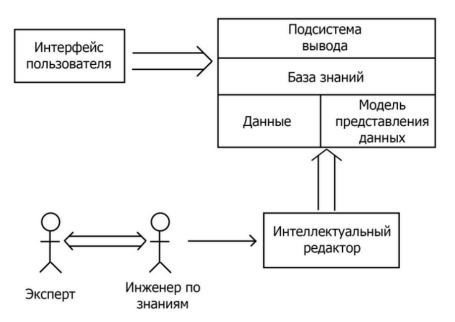
\includegraphics[width=0.75\textwidth]{1.png}
    \caption{Структура экспертной системы.}
    \label{fig1}
\end{figure}

Экспертная система работает в двух основных режимах. Первый режим --- режим приобретения знаний. В нём база знаний формируется на основе выбранных источников и характеристик объектов. Второй режим --- режим решения задачи, или режим консультации. В нём пользователь взаимодействует с системой, отвечает на вопросы и получает итоговый результат.

\subsection{Продукционная модель}

В качестве модели представления знаний используется продукционная модель. Продукционная система включает в себя три компоненты:

\begin{enumerate}
    \item набор правил, или продукций, представляющих базу знаний;
    \item рабочую память, в которой хранятся исходные факты и факты, полученные в процессе вывода;
    \item механизм логического вывода, применяющий правила к имеющимся фактам.
\end{enumerate}

В основе продукционной модели находится продукция, то есть правило вида:

\[
\text{ЕСЛИ } \langle \text{условие} \rangle
\text{ ТО } \langle \text{действие}1 \rangle
\text{ ИНАЧЕ } \langle \text{действие}2 \rangle.
\]

Условие правила называется антецедентом, а действие --- консеквентом. Условия могут объединяться с помощью логических связок AND и OR. Правило срабатывает, если при сопоставлении фактов, находящихся в рабочей памяти, с антецедентом правила обнаруживается совпадение. После этого результат выполнения правила заносится в рабочую память.

Структура правил продукционной модели изображена на рис. \ref{2}.

\begin{figure}[H]
    \centering
    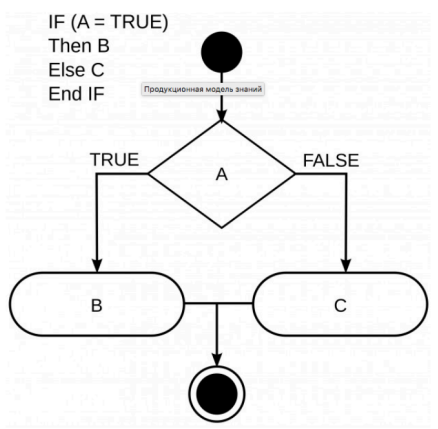
\includegraphics[width=0.75\textwidth]{2.png}
    \caption{Структура правил продукционной модели.}
    \label{2}
\end{figure}

В данной экспертной системе продукционная модель используется для обхода бинарного дерева решений.

Правило для внутреннего узла можно записать следующим образом:

\[
\begin{aligned}
&\text{ЕСЛИ пользователь находится в узле } Q_i1 \\
&\text{И ответ пользователя равен } yes, \\
&\text{ТО выполнить переход в узел } yes-next(Q_i2) \\
&\text{ИНАЧЕ выполнить переход в узел} no-next(Q_i3)
\end{aligned}
\]

Для конечного узла (листа) правило имеет вид:

\[
\begin{aligned}
&\text{ЕСЛИ достигнут лист } R_j, \\
&\text{ТО вывести соответствующее заключение и завершить работу.}
\end{aligned}
\]


\subsection{Структура бинарного дерева}

Бинарное дерево решений представляет собой ориентированное дерево, в котором каждый узел имеет ровно два потомка: по веткам "да" и "нет".

Структура бинарного дерева решений экспертной системы представлена на рис. \ref{3}, рис. \ref{4}, рис. {5} и рис. {6}.

\begin{figure}[H]
    \centering
    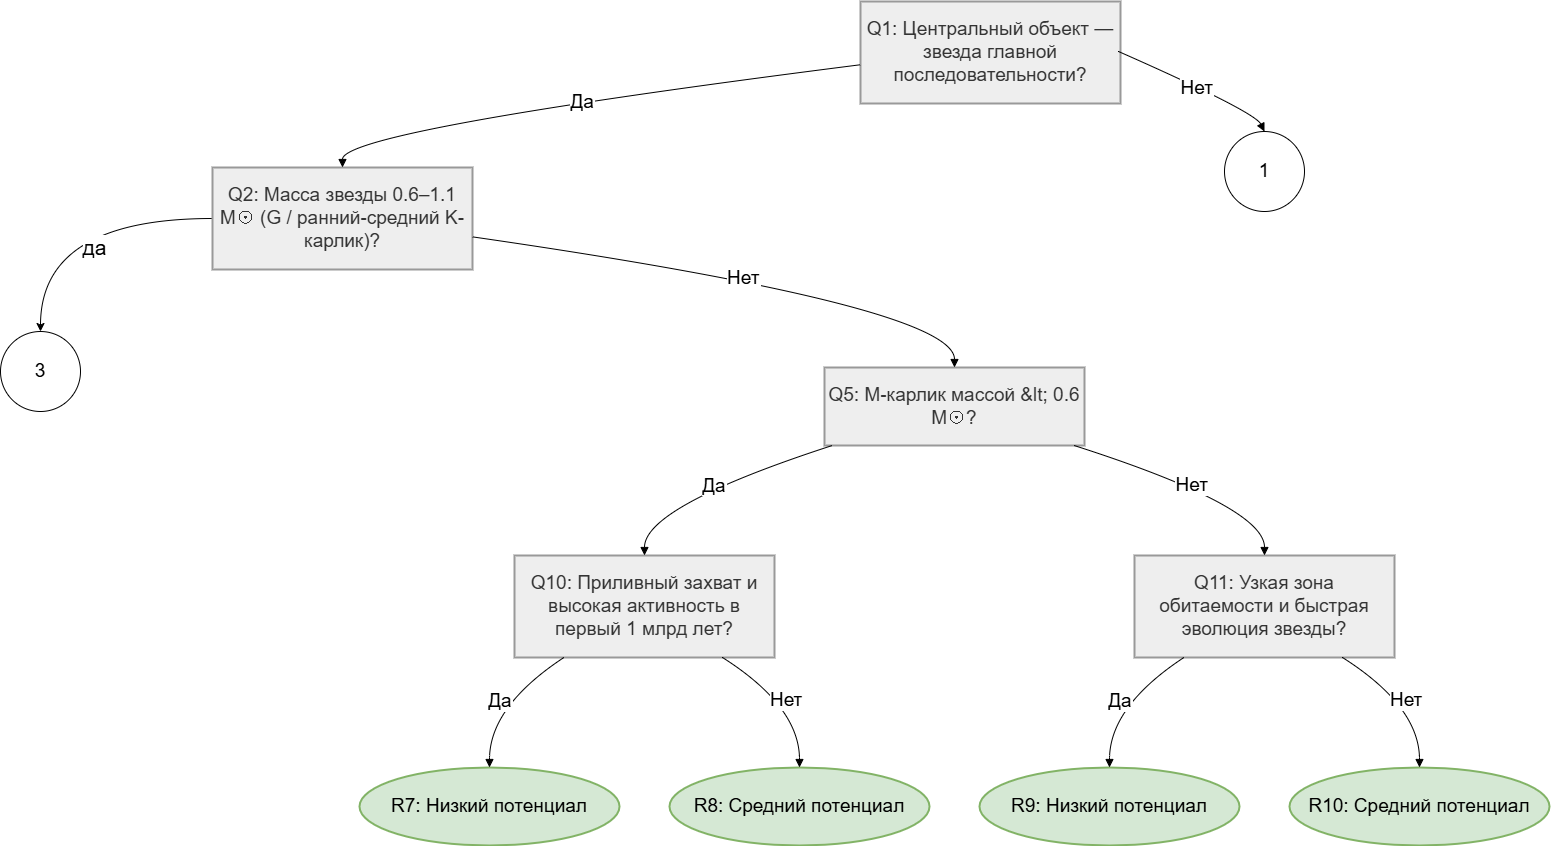
\includegraphics[width=1\textwidth]{5.png}
    \caption{Бинарное дерево решений (часть 1).}
    \label{3}
\end{figure}

\begin{figure}[H]
    \centering
    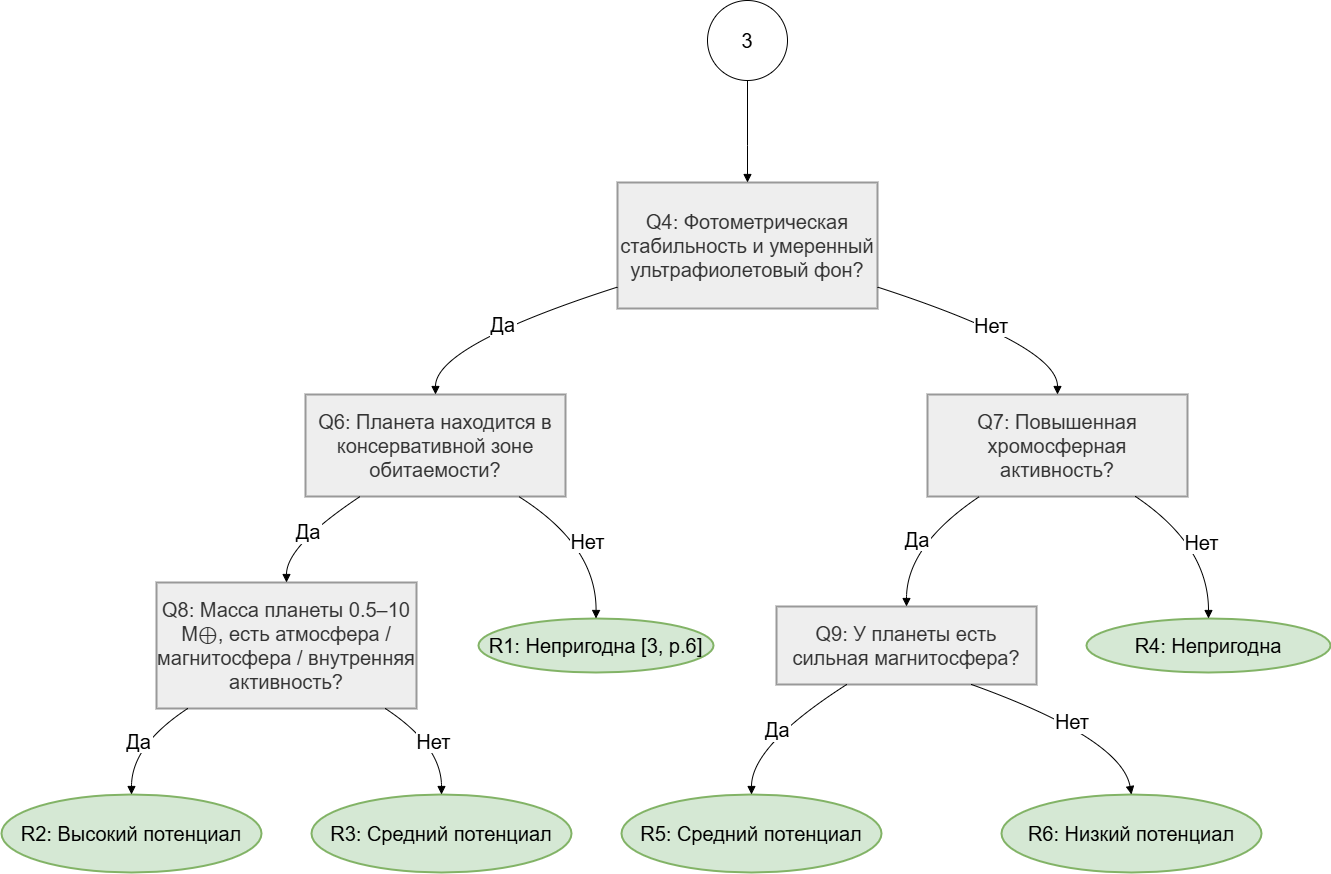
\includegraphics[width=1\textwidth]{6.png}
    \caption{Бинарное дерево решений (часть 2).}
    \label{4}
\end{figure}

\begin{figure}[H]
    \centering
    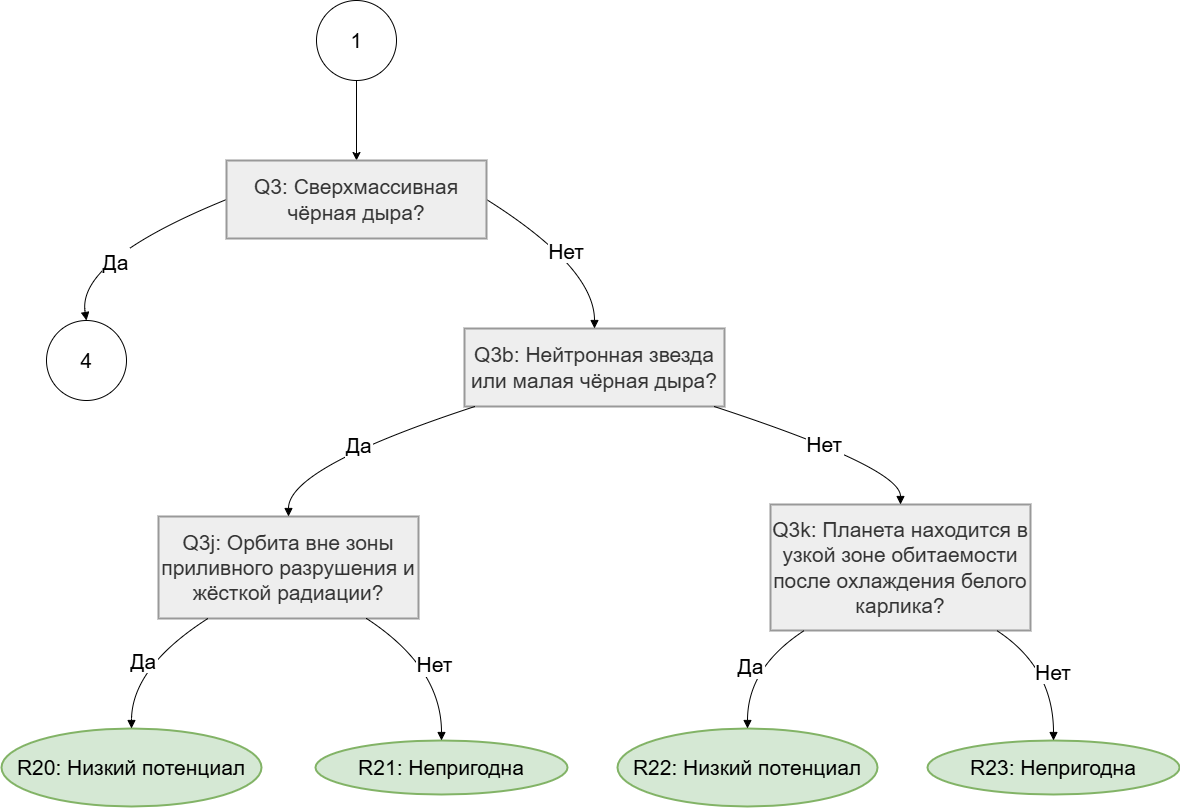
\includegraphics[width=1\textwidth]{7.png}
    \caption{Бинарное дерево решений (часть 3).}
    \label{5}
\end{figure}

\begin{figure}[H]
    \centering
    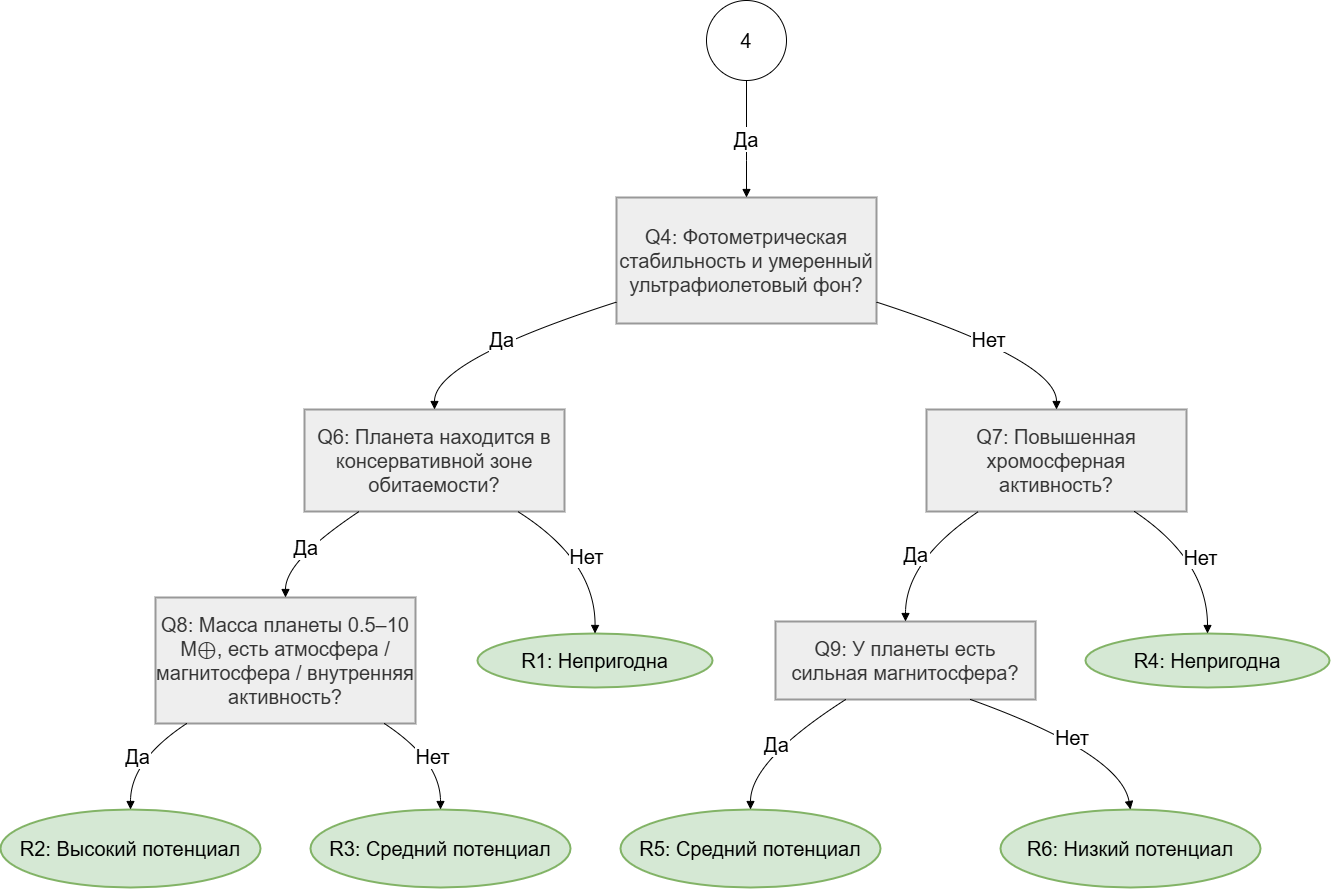
\includegraphics[width=1\textwidth]{8.png}
    \caption{Бинарное дерево решений (часть 4).}
    \label{6}
\end{figure}

Построенное дерево решений имеет следующие параметры:

\begin{table}[H]
\centering
\caption{Параметры бинарного дерева решений}
\begin{tabularx}{0.9\textwidth}{>{\raggedright\arraybackslash}X c}
\toprule
\textbf{Параметр} & \textbf{Значение} \\
\midrule
Количество правил & 17 \\
Количество фактов & 18 \\
Общее количество узлов & 35 \\
Количество переходов между узлами & 34 \\
Количество уровней дерева & 6 \\
Минимальное количество ответов до результата & 3 \\
Максимальное количество ответов до результата & 5 \\
Количество различных итоговых заключений & 4 \\
\bottomrule
\end{tabularx}
\end{table}

\subsection{Механизм логического вывода}

Механизм логического вывода состоит в анализе имеющихся фактов и применении к ним правил из базы знаний для получения нового факта (узел) или конечного результата (лист).

Алгоритм следующий:

\begin{enumerate}
    \item в рабочую память помещается начальный факт, указывающий на корневое правило;
    \item система находит описание текущего правила в базе знаний;
    \item пользователю выводится текст вопроса;
    \item пользователь вводит ответ;
    \item система проверяет корректность ответа;
    \item в зависимости от ответа выбирается следующая вершина дерева;
    \begin{itemize}
        \item если следующая вершина является правилом, процесс повторяется;
        \item если следующая вершина является фактом, система выводит заключение, а работа программы завершается.
    \end{itemize}
\end{enumerate}

\newpage

\section{Особенности реализации}

\subsection{Среда CLIPS}

Для реализации экспертной системы была выбрана среда CLIPS. CLIPS является одним из языков построения экспертных систем, основанных на продукционной модели представления знаний. 

В реализованной системе CLIPS используется для хранения базы знаний, организации рабочей памяти, обработки пользовательских ответов и выполнения переходов между узлами бинарного дерева, а также для взаимодействия с пользователем (получение ответов пользователя и возврат следующего узла дерева).

\subsection{Представление данных}

В программе используются шаблоны фактов, задаваемые с помощью конструкции \texttt{deftemplate}. Они описывают структуру данных, которые помещаются в рабочую память CLIPS.

Основными шаблонами являются:

\begin{itemize}
    \item \texttt{answer} --- хранит ответ пользователя на вопрос;
    \item \texttt{question} --- описывает правило;
    \item \texttt{result} --- описывает факт;
    \item \texttt{ask} --- указывает, какой вопрос необходимо задать;
    \item \texttt{route} --- задаёт переход к следующему узлу;
    \item \texttt{conclusion} --- хранит итоговое заключение.
\end{itemize}

Например, шаблон вопроса имеет следующую структуру:

\begin{Code}
(deftemplate question
  (slot id (type SYMBOL))
  (slot text (type STRING))
  (slot yes-next (type SYMBOL))
  (slot no-next (type SYMBOL))
)
\end{Code}

Поле \texttt{id} содержит идентификатор правила. Поле \texttt{text} хранит текст, выводимый пользователю. Поля \texttt{yes-next} и \texttt{no-next} задают идентификаторы узлов, к которым система должна перейти при ответах "да" и "нет" соответственно.

\subsection{Функция обработки пользовательского ввода}

Для ввода ответов используется функция \texttt{ask-yes-no}. Она выводит пользователю текст вопроса, считывает строку ответа, приводит её к нижнему регистру и проверяет, относится ли введённое значение к допустимым вариантам.

Функция принимает следующие варианты ответов в любом регистре:

\begin{itemize}
    \item положительные ответы: \texttt{да}, \texttt{д}, \texttt{yes}, \texttt{y};
    \item отрицательные ответы: \texttt{нет}, \texttt{н}, \texttt{no}, \texttt{n}.
\end{itemize}

Если пользователь вводит некорректное значение, система повторно запрашивает ответ.

Вход: строка (сообщение пользователя).

Выход: сообщение пользователя после парсинга или приглашение ввести ответ снова в корректной форме.

Код:

\begin{Code}
(deffunction ask-yes-no (?text)
  (bind ?resp "")

  (while TRUE do
    (printout t ?text crlf "Введите ответ (да/нет): ")
    (bind ?resp (lowcase (readline)))

    (if (or (eq ?resp "да") (eq ?resp "д") 
            (eq ?resp "yes") (eq ?resp "y"))
      then
      (return yes))

    (if (or (eq ?resp "нет") (eq ?resp "н") 
            (eq ?resp "no") (eq ?resp "n"))
      then
      (return no))

    (printout t "Некорректный ввод." crlf crlf)
  )
)
\end{Code}

\subsection{База знаний}

База знаний экспертной системы задаётся с помощью конструкции \texttt{deffacts}. В ней перечислены все правила дерева и все возможные факты. Также в базе знаний задаётся начальное правило:

\begin{Code}
(ask (id Q1))
\end{Code}

Этот факт указывает системе, что первым должен быть задан вопрос правила с идентификатором \texttt{Q1}, т.е. определяется корень бинарного дерева решений.

Пример описания вопроса в базе знаний:

\begin{Code}
(question
  (id Q1)
  (text "Центральный объект - звезда главной последовательности?")
  (yes-next Q2)
  (no-next Q3))
\end{Code}

В данном примере, если пользователь отвечает на этот вопрос положительно, система переходит к правилу \texttt{Q2}, а если ответ отрицательный, выполняется переход к правилу \texttt{Q3}.

Пример описания конечного результата:

\begin{Code}
(result (id R2) (text "Высокий потенциал"))
\end{Code}

\subsection{Правила продукционной системы}

В программе используется несколько универсальных правил, управляющих работой экспертной системы.

Правило \texttt{ask-question} отвечает за вывод вопроса пользователю, получение ответа и формирование факта перехода:

Вход: ID правила, вопрос которого нужно задать.

Выход: вопрос правила, который нужно задать.

Код:

\begin{Code}
(defrule ask-question
  ?a <- (ask (id ?qid))
  (question (id ?qid) (text ?text) 
            (yes-next ?yes-next) 
            (no-next ?no-next))
  =>
  (retract ?a)
  (bind ?prompt (str-cat ?qid ": " ?text))
  (bind ?resp (ask-yes-no ?prompt))
  (assert (answer (question ?qid) (response ?resp)))

  (if (eq ?resp yes)
    then
    (bind ?next ?yes-next)
    else
    (bind ?next ?no-next))

  (assert (route (target ?next)))
)
\end{Code}

После получения ответа система создаёт факт \texttt{route}, содержащий идентификатор следующего узла. 

Итоговый вывод выполняется правилом \texttt{print-conclusion}:

Вход: вывод, который нужно вывести.

Выход: печать вывода на экран.

Код: 

\begin{Code}
(defrule print-conclusion
  ?c <- (conclusion (text ?text))
  =>
  (retract ?c)
  (printout t crlf "Заключение: " ?text crlf)
)
\end{Code}

\subsection{Логика работы экспертной системы}

Работа реализованной экспертной системы происходит последовательно. После запуска в рабочей памяти находится факт \texttt{ask} с идентификатором начального правила. Затем система извлекает соответствующее правило из базы знаний, выводит его пользователю и ожидает ответ.

В зависимости от ответа выбирается одна из двух ветвей дерева. Если выбранный узел является правилом, следующим шагом будет вывод нового вопроса пользователю и ожидание от него ответа. Если выбранный узел является фактом, система выводит итоговую оценку и программа завершает работу.

Алгоритм работы программы:

Вход: ответы пользователя на заданный ему вопрос.

Выход: оценка потенциальной обитаемости планеты.

\begin{enumerate}
    \item запуск программы;
    \item загрузка базы знаний;
    %\item запуск механизма вывода CLIPS;
    \item активация начального правила \texttt{Q1};
    \item вывод вопроса пользователю;
    \item получение и проверка ответа;
    \item выбор следующего узла дерева;
    \item если это правило, пункт 4; если это факт, пункт 8;
    \item вывод конечного результата,
    \item завершение программы
\end{enumerate}

\newpage

\section*{Заключение}
\addcontentsline{toc}{section}{Заключение}

В результате выполнения курсовой работы была разработана экспертная система оценки потенциальной обитаемости планеты. Система реализована в среде CLIPS и использует продукционную модель представления знаний. Логика принятия решений организована в виде бинарного дерева, узлы которого соответствуют правилам (т.е. вопросам), а листья --- фактам (т.е. итоговой оценке).

Были выполнены следующие шаги:

\begin{enumerate}
  \item Была изучена предметная область.
  \begin{itemize}
    \item Было выяснено, какими могут быть центральные объекты систем.
    \item Были изучены критерии, по которым можно оценить потенциальную обитаемость планеты, для каждого центрального объекта системы.
  \end{itemize}
  \item Было построено бинарное дерево решений.
  \begin{itemize}
    \item Дерево содержит 6 ярусов.
    \item Дерево содержит 35 узлов.
    \item Факты, описанные в дереве, обоснованы авторитетными источниками; ссылки на источники даны в разделе \hyperref[lit]{Список литературы}.
  \end{itemize}
  \item Была реализована программа в среде CLIPS.
  \begin{itemize}
    \item Было реализовано 17 правил.
    \item Было реализовано 18 фактов.
    \item Были реализованы шаблоны и функции, необходимые для взаимодействия с пользователем и продвижению по дереву.
    \item Была реализована устойчивость к некорректному вводу пользователя путём вывода сообщения с уведомлением о некорректном вводе и повторного запроса ввода в случае некорректного ввода.
  \end{itemize}
\end{enumerate}

Разработанное бинарное дерево включает 17 правил и 18 фактов. Итоговые результаты сведены к четырём видам: высокий потенциал, средний потенциал, низкий потенциал и непригодность.

Достоинства программы:

\begin{itemize}
    \item база знаний системы является полной в рамках предметной области, рассматриваемой в ней;
    \item отделение базы знаний от правил логического вывода, что позволяет удобно добавлять новые знания без изменения правил вывода;
    \item возможность обработки некорректного пользовательского ввода;
    \item поддержку русских и английских вариантов ответов;
    \item сложность алгоритма --- $\log(N)$.
\end{itemize}

Недостатки программы:

\begin{itemize}
    \item отсутствие графического интерфейса;
    \item программа не допускает ответа "не знаю" или его аналогов, из чего следует, что пользователь должен знать ответ на каждый задаваемый ему вопрос, чтобы получить результат;
    \item реальные астрофизические условия сложнее, чем в данной модели: если экспертная система сделает вывод, что планета потенциально обитаема, на самом деле может оказаться, что она непригодна для жизни из-за других условий (например, характеристик самой планеты, а не объектов вокруг неё).
    \item при добавлении новых правил необходимо перестраивать всю часть дерева, идущую после добавленного правила.
\end{itemize}

Масштабируемость:

\begin{itemize}
    \item добавление графического интерфейса;
    \item расширение базы знаний;
    \item упрощение процесса добавления новых знаний (например, через графический интерфейс);
    \item добавление поддержки ответа "не знаю": вопрос, на который пользователь не знает овтета, пропускается, и он отвечает на все вопросы, следующие из этого (например, планета может оказаться непригодна, основываясь на одном из ответов пользователя, независимо от ответов до этого вопроса);
    \item добавление поддержки обратного логического вывода.
\end{itemize}

Возможное развитие работы может включать расширение базы знаний, добавление режима неопределённого ответа, введение весовых коэффициентов для различных факторов, использование численных параметров планет и звёзд, а также создание графического интерфейса пользователя. Кроме того, систему можно дополнить модулем объяснения, который будет показывать пользователю путь по дереву и причины получения конкретного заключения.

Таким образом, разработанная программа демонстрирует применение методов теории графов, продукционных моделей и экспертных систем для решения задачи качественной оценки потенциальной обитаемости планет.

\newpage

\begin{thebibliography}{9}
\label{lit}

    \bibitem{hand} Michael Perryman. Exoplanet Handbook / Michael Perryman --- 2-е изд. --- Кембридж: 2011.--- 3823 с.

	\bibitem{miller} Life on Miller's Planet: The Habitable Zone Around Supermassive Black holes [Электронный ресурс]. --- URL: \url{https://arxiv.org/abs/1910.00940} (дата обращения: 21.04.2026).

    \bibitem{neutron} Neutron Star Planets: Atmospheric processes and habitability [Электронный ресурс]. --- URL: \url{https://arxiv.org/abs/1705.07688} (дата обращения: 21.04.2026).

    \bibitem{tele} Секция <<Телематика>> [Электронный ресурс]. --- URL: \url{https://tema.spbstu.ru/tgraph/} (дата обращения: 11.05.2026).

\end{thebibliography}

\newpage

\section*{Приложение. Реализация экспертной системы в среде CLIPS}
\addcontentsline{toc}{section}{Приложение. Реализация экспертной системы в среде CLIPS}
\begin{Code}
(deftemplate answer
  (slot question (type SYMBOL))
  (slot response (type SYMBOL) (allowed-symbols yes no))
)

(deftemplate question
  (slot id (type SYMBOL))
  (slot text (type STRING))
  (slot yes-next (type SYMBOL))
  (slot no-next (type SYMBOL))
)

(deftemplate result
  (slot id (type SYMBOL))
  (slot text (type STRING))
)

(deftemplate ask
  (slot id (type SYMBOL))
)

(deftemplate route
  (slot target (type SYMBOL))
)

(deftemplate conclusion
  (slot text (type STRING))
)

(deffunction ask-yes-no (?text)
  (bind ?resp "")

  (while TRUE do
    (printout t ?text crlf "Введите ответ (да/нет): ")
    (bind ?resp (lowcase (readline)))

    (if (or (eq ?resp "да") (eq ?resp "д") (eq ?resp "yes") (eq ?resp "y"))
      then
      (return yes))

    (if (or (eq ?resp "нет") (eq ?resp "н") (eq ?resp "no") (eq ?resp "n"))
      then
      (return no))

    (printout t "Некорректный ввод. Пожалуйста, введите \"да\" или \"нет\"." crlf crlf)
  )
)

(deffacts knowledge-base
  (question
    (id Q1)
    (text "Центральный объект — звезда главной последовательности?")
    (yes-next Q2)
    (no-next Q3))
  (question
    (id Q2)
    (text "Масса звезды 0.6–1.1 M☉ (G / ранний-средний K-карлик)?")
    (yes-next Q4)
    (no-next Q5))
  (question
    (id Q3)
    (text "Сверхмассивная чёрная дыра?")
    (yes-next Q3a)
    (no-next Q3b))
  (question
    (id Q4)
    (text "Фотометрическая стабильность и умеренный ультрафиолетовый фон?")
    (yes-next Q6)
    (no-next Q7))
  (question
    (id Q5)
    (text "M-карлик массой < 0.6 M☉?")
    (yes-next Q10)
    (no-next Q11))
  (question
    (id Q6)
    (text "Планета находится в консервативной зоне обитаемости?")
    (yes-next Q8)
    (no-next R1))
  (question
    (id Q7)
    (text "Повышенная хромосферная активность?")
    (yes-next Q9)
    (no-next R4))
  (question
    (id Q8)
    (text "Масса планеты 0.5–10 M⊕, есть атмосфера / магнитосфера / внутренняя активность?")
    (yes-next R2)
    (no-next R3))
  (question
    (id Q9)
    (text "У планеты есть сильная магнитосфера?")
    (yes-next R5)
    (no-next R6))
  (question
    (id Q10)
    (text "Приливный захват и высокая активность в первый 1 млрд лет?")
    (yes-next R7)
    (no-next R8))
  (question
    (id Q11)
    (text "Узкая зона обитаемости и быстрая эволюция звезды?")
    (yes-next R9)
    (no-next R10))
  (question
    (id Q3a)
    (text "Спин чёрной дыры экстремальный (a/M≈1)?")
    (yes-next Q3c)
    (no-next R11))
  (question
    (id Q3b)
    (text "Нейтронная звезда или малая чёрная дыра?")
    (yes-next Q3j)
    (no-next Q3k))
  (question
    (id Q3c)
    (text "Значительное замедление времени?")
    (yes-next Q3d)
    (no-next R12))
  (question
    (id Q3d)
    (text "Блюшифт фонового излучения создаёт полезный поток энергии?")
    (yes-next R13)
    (no-next R14))
  (question
    (id Q3j)
    (text "Орбита вне зоны приливного разрушения и жёсткой радиации?")
    (yes-next R20)
    (no-next R21))
  (question
    (id Q3k)
    (text "Планета находится в узкой зоне обитаемости после охлаждения белого карлика?")
    (yes-next R22)
    (no-next R23))

  (result (id R1) (text "Непригодна"))
  (result (id R2) (text "Высокий потенциал"))
  (result (id R3) (text "Средний потенциал"))
  (result (id R4) (text "Непригодна"))
  (result (id R5) (text "Средний потенциал"))
  (result (id R6) (text "Низкий потенциал"))
  (result (id R7) (text "Низкий потенциал"))
  (result (id R8) (text "Средний потенциал"))
  (result (id R9) (text "Низкий потенциал"))
  (result (id R10) (text "Средний потенциал"))
  (result (id R11) (text "Низкий потенциал"))
  (result (id R12) (text "Непригодна"))
  (result (id R13) (text "Низкий потенциал"))
  (result (id R14) (text "Непригодна"))
  (result (id R20) (text "Низкий потенциал"))
  (result (id R21) (text "Непригодна"))
  (result (id R22) (text "Низкий потенциал"))
  (result (id R23) (text "Непригодна"))

  (ask (id Q1))
)

(defrule ask-question
  ?a <- (ask (id ?qid))
  (question (id ?qid) (text ?text) (yes-next ?yes-next) (no-next ?no-next))
  =>
  (retract ?a)

  (if (eq ?qid Q1)
    then
    (printout t crlf
      "Экспертная система оценки потенциальной обитаемости планеты." crlf
      "Отвечайте на вопросы словами \"да\" или \"нет\"." crlf))

  (bind ?prompt (str-cat ?qid ": " ?text))
  (bind ?resp (ask-yes-no ?prompt))
  (assert (answer (question ?qid) (response ?resp)))

  (if (eq ?resp yes)
    then
    (bind ?next ?yes-next)
    else
    (bind ?next ?no-next))

  (assert (route (target ?next)))
)

(defrule route-to-question
  ?r <- (route (target ?target))
  (question (id ?target))
  =>
  (retract ?r)
  (assert (ask (id ?target)))
)

(defrule route-to-result
  ?r <- (route (target ?target))
  (result (id ?target) (text ?text))
  =>
  (retract ?r)
  (assert (conclusion (text ?text)))
)

(defrule print-conclusion
  ?c <- (conclusion (text ?text))
  =>
  (retract ?c)
  (printout t crlf "Заключение: " ?text crlf)
)
\end{Code}


\end{document}